\documentclass[fr]{../../../../../../eplexam}
\usepackage{amsmath}
\usepackage{tikz}
\usepackage{enumitem}

\newcommand{\rang}{\mathrm{rang}}

\usetikzlibrary{shapes,arrows,positioning,calc}
\tikzset{
	block/.style = {draw, fill=white, rectangle, minimum height=3em, minimum width=3em},
	sum/.style = {draw, fill=white, circle, node distance=1cm},
	input/.style = {coordinate},
	output/.style = {coordinate},
	pinstyle/.style = {pin edge={to-, thin, black}}
}

\hypertitle{sigsys-FSAB1106}{4}{FSAB}{1106}{2017}{Juin}
{Jean-Martin Vlaeminck}
{Luc Vandendorpe et Vincent Wertz}

\section{LV1}
Soit un système linéaire permanent (c-à-d invariant dans le temps) de réponse impulsionnelle $h(t)$ et de réponse en fréquence $H(j\omega)$.
On sait par ailleurs que le système est \emph{réel}.

On introduit $x(t) = \sin (\omega_0 t + \phi)$ dans ce système. Que vaut le signal qui est produit en sortie ? Démontrer le résultat.

\begin{solution}
On a
\[ x(t) = \sin (\omega_0 t + \phi) = \frac{e^{j(\omega_0 t + \phi)} - e^{-j(\omega_0 t + \phi)}}{2j} \]
et donc, la transformée de Fourier du signal est
\[ x(t) \leftrightarrow X(j\omega) = \frac{\pi}{j} e^{j\phi} \delta(\omega-\omega_0) - \frac{\pi}{j} e^{-j\phi} \delta(\omega+\omega_0)\]
Dès lors,
\begin{align*}
Y(j\omega) &= H(j\omega) \cdot X(j\omega) \\
&= H(j\omega) \cdot \left( \frac{\pi}{j} e^{j\phi} \delta(\omega - \omega_0) - \frac{\pi}{j} e^{-j\phi} \delta(\omega + \omega_0) \right) \\
&= H(j\omega_0) \frac{\pi}{j} e^{j\phi} \delta(\omega - \omega_0) - H(-j\omega_0) \frac{\pi}{j} e^{-j\phi} \delta(\omega + \omega_0) \\
&= \abs{H(j\omega_0)} \frac{\pi}{j} e^{j\phi} e^{j \arg(H(j\omega_0))} \delta(\omega-\omega_0) - \abs{H(-j\omega_0)} \frac{\pi}{j} e^{-j\phi} e^{j\arg( H(-j\omega_0))} \delta(\omega+\omega_0) \\
&= \abs{H(j\omega_0)} \frac{\pi}{j} e^{j\phi} e^{j \arg(H(j\omega_0))} \delta(\omega-\omega_0) - \abs{H(j\omega_0)} \frac{\pi}{j} e^{-j\phi} e^{-j\arg( H(j\omega_0))} \delta(\omega+\omega_0) \\
&= \abs{H(j\omega_0)} \left( \frac{\pi}{j} e^{j (\phi + \arg(H(j\omega_0)))} \delta(\omega-\omega_0) - \frac{\pi}{j} e^{-j(\phi + \arg(H(j\omega_0)))} \delta(\omega+\omega_0) \right) \\
\end{align*}
dont la transformée inverse est
\begin{align*}
Y(j\omega) \leftrightarrow y(t) &= \abs{H(j\omega_0)} \frac{e^{j (\omega_0 t + \phi + \arg(H(j\omega_0))} - e^{-j (\omega_0 t + \phi + \arg(H(j\omega_0)))}}{2j} \\
&= \abs{H(j\omega_0)} \sin (\omega_0 t + \phi + \arg(H(j\omega_0))) \\
\end{align*}
un résultat bien connu, et relativement logique : le signal de départ est déphasé de $\arg(H(j\omega_0))$, et est multiplié par $\abs{H(j\omega_0)}$.

Rappelons que, pour un système réel, la partie réelle de la fonction de transfert est paire et la partie imaginaire est impaire, ce qui a pour conséquence que le module est pair et l'argument est impair.
\end{solution}

\section{LV2}
On s'intéresse à la transformée de Fourier discrète (TFD) d'un vecteur $X$ de taille $N = 8$ comprenant les échantillons d'un signal $x[n]$ \emph{réel}, pour $n = 0, \dots, N-1$.

La TFD produit un vecteur $Y = [Y[0], \dots, Y[N-1]]^T$
\begin{enumerate}[label=(\alph*)]
	\item Sachant que la période d'échantillonnage du signal temporel est $T$, quelles sont les positions des échantillons $Y[k]$ (en fréquences vraies, c-à-d en hertz) ? Justifier.
	\item Sachant que le signal $x[n]$ de départ est réel, quelles sont les propriétés ou liens dont bénéficient les coefficients $X[k]$ des produits ?
\end{enumerate}

Remarque : l'énoncé de cette question est incomplet, notamment la démonstration qu'il fallait faire.

\nosolution

\section{LV3}
On génère un signal périodique $x(t) = \sin (2 \pi f_0 t)$. Ce signal est d'abord échantillonné par un échantillonneur\footnote{Sans blague ?} qui fonctionne à la fréquence $f_e$. Ensuite, le résultat de l'échantillonnage est interpolé par un filtre réel, fonctionnant en temps continu de type passe-bas (?) idéal et de fréquence de coupure $f_e/2$ (il laisse donc passer toutes les fréquences $f$ telles que $\abs{f} \le f_e/2$).%FIXME < ou <= ?
Le schéma complet est décrit ci-dessous.
%\begin{center}
%	\begin{tikzpicture}
%	%TODO
%	\end{tikzpicture}
%\end{center}
\begin{enumerate}[label=(\alph*)]
	\item Représentez graphiquement le spectre du signal obtenu en sortie du filtre analogique lorsque $f_0 = f_e/4$. Justifiez.
	\item Pareil lorsque $f_0 = 7f_e/8$. Justifiez.
	\item Représentez graphiquement le spectre du signal obtenu en sortie du filtre analogique lorsque, à $f_e$ fixé, on augmente $f_0$ de $0$ jusque $3f_e/2$. Justifiez.
\end{enumerate}

\nosolution

\section{VW1}
On considère un système causal décrit par la fonction de transfert
\[G(s) = \frac{s+1}{(s-1)(s^2 + \frac{3}{2} s + 1)}\]
\begin{enumerate}[label=(\alph*)]
	\item Ce système est-il stable EBSB ?
	\item Est-il possible de concevoir un système de fonctions de transfert $H(s)$ dont le degré du numérateur est inférieur au degré du dénominateur et tel que la connexion en série représentée ci-dessous soit stable ?
	\begin{center}
		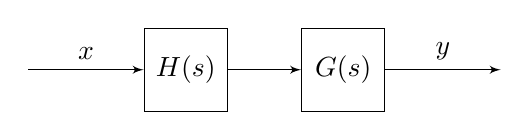
\begin{tikzpicture}[auto, node distance=2cm, >=latex']
		\node [input, name=input] {$x$};
		\node [block, right of=input] (htf) {$H(s)$};
		\node [block, right of=htf] (gtf) {$G(s)$};
		\node [output, right of=gtf] (output) {$y$};
		\draw [->] (input) -- node {$x$} (htf);
		\draw [->] (htf) -- (gtf);
		\draw [->] (gtf) -- node[name=y] {$y$} (output);
		\end{tikzpicture}
	\end{center}
	\item Proposer un tel système.
	\item Est-il possible de trouver un gain $K$ tel que le feedback représenté à la figure suivante donne lieu à une fonction de transfert stable ? Quelles sont les éventuelles conditions sur $K$ ?
	\begin{center}
		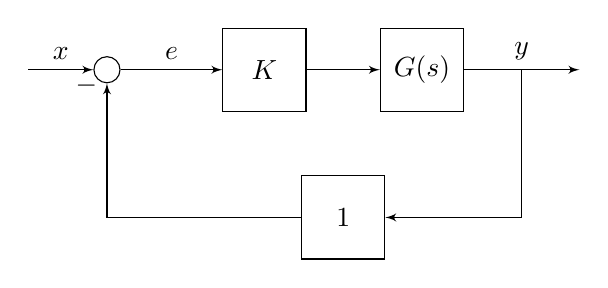
\begin{tikzpicture}[auto, node distance=2cm, >=latex']
			\node [input, name=input] {$x$};
			\node [sum, right of=input] (sum) {};
			\node [block, right of=sum] (factor) {$K$};
			\node [block, right of=factor] (tf) {$G(s)$};
			\node [output, right of=tf] (output) {$y$};
			\draw [->] (factor) -- node[name=u] {} (tf);
			\node [block, below of=u] (one) {$1$};
			\draw [->] (input) -- node {$x$} (sum);
			\draw [->] (sum) -- node {$e$} (factor);
			\draw [->] (tf) -- node[name=y] {$y$} (output);
			\draw [->] (y) |- (one);
			\draw [->] (one) -| node[pos=0.99] {$-$} (sum);
		\end{tikzpicture}
	\end{center}
	\item Si le but est de stabiliser la fonction de transfert, quel schéma semble préférable et pourquoi ?
\end{enumerate}

\begin{solution}
\begin{enumerate}[label=(\alph*)]
	\item Les pôles de la fonction de transfert sont en $1$, en $-\frac{3}{4} + i\frac{\sqrt{7}}{2}$ et en $-\frac{3}{4} - i\frac{\sqrt{7}}{2}$. Comme $1$ est à droite de l'axe imaginaire, et que le système est causal, le système n'est pas stable BIBO (il faudrait que tous les pôles soient à gauche de l'axe imaginaire, donc à partie réelle négative).
	\item Pour cela, il faut une fonction de transfert dont le numérateur élimine le pôle à partie réelle positive, et dont les pôles soient à partie réelle négative. Par exemple,
	\[H(s) = \frac{s-1}{(s+1)(s+2)}\]
	%FIXME pas sûr
	\item La fonction de transfert du système complet s'obtient en écrivant que
	\[ Y(s) = K G(s) (X(s)-Y(s)) \]
	ce qui donne
	\[ \frac{Y(s)}{X(s)} = \frac{K G(s)}{1+K G(s)} \]
	soit
	\begin{align*}
	\frac{Y(s)}{X(s)} &= \frac{K \frac{s+1}{(s-1) \left(s^2 + \frac{3}{2}s + 1\right)}}{1+K \frac{s+1}{(s-1)\left(s^2 + \frac{3}{2}s + 1\right)}} \\
	&= \frac{K (s+1)}{s^3 + \frac{1}{2}s^2 - \frac{1}{2}s - 1 + Ks + K}
	\end{align*}
	Pour que la fonction de transfert soit stable, il faut donc s'assurer que le dénominateur ne contienne pas de racines à partie réelle positive. Pour cela, on utilise le critère de Routh-Hurwitz sur le polynôme $s^3 + \frac{1}{2} s^2 + (K - \frac{1}{2}) s + (K-1)$ :
	
	\begin{center}
	\begin{tabular}{ccc}
	$1$ & $K-\frac{1}{2}$ & \dots \\
	$\frac{1}{2}$ & $K-1$ & \dots \\
	$K - \frac{1}{2} - \frac{K-1}{\frac{1}{2}} = -K +\frac{3}{2}$ & 0 & \dots \\
	$K - 1$ & 0 & \dots \\
	0 & 0 & \dots \\
	\end{tabular}
	\end{center}

	Le critère de Routh-Hurwitz stipule que le nombre de racines à partie réelle positive est égal au nombre de changement de signe des nombres de la première colonne. Comme on veut déterminer l'ensemble des $K$ tels que toutes les racines ont des parties réelles négatives, il faut que tous les nombres de la première colonne soient strictement positifs, et donc il faut que
	\[
	\begin{cases}
	\frac{3}{2} - K > 0 \Rightarrow K < \frac{3}{2} \\
	K - 1 > 0 \Rightarrow K > 1 \\
	\end{cases}
	\]
	et donc,
	\[ 1 < K < \frac{3}{2} \]
	\item On préfère en général la solution avec feedback, car elle n'introduit pas de pôles supplémentaires, et a un impact contrôlable sur le gain du système. % FIXME
\end{enumerate}
\end{solution}

\section{VW2}
On considère le système causal décrit par les équations d'état suivantes
\begin{align*}
q[n+1] &= \begin{pmatrix} \frac{1}{2} & 0 & 1 \\ 0 & 1 & \frac{5}{2} \\ 0 & \frac{1}{2} & \frac{3}{4} \end{pmatrix} q[n] + \begin{pmatrix} 1 \\ 0 \\ 0 \end{pmatrix} x[n] \\
y[n] &= \begin{pmatrix} 1 & 0 & 1 \end{pmatrix} q[n] \\
\end{align*}
\begin{enumerate}[label=(\alph*)]
	\item Le système est-il stable de manière interne ?
	\item Le système est-il commandable ?
	\item Le système est-il observable ?
	\item Calculer la réponse impulsionnelle du système.
	\item Le système est-il stable EBSB ?
\end{enumerate}

\begin{solution}
\begin{enumerate}
	\item Pour cela, on calcule les valeurs propres de la matrice $A$ du système :
	\begin{align*}
	\begin{vmatrix}
	\lambda - \frac{1}{2} & 0 & -1 \\
	0 & \lambda - 1 & -\frac{5}{2} \\
	0 & -\frac{1}{2} & \lambda - \frac{3}{4} \\
	\end{vmatrix}
	&= \left(\lambda - \frac{1}{2}\right) \left( (\lambda - 1) \left(\lambda - \frac{3}{4}\right)  - \frac{5}{2} \frac{1}{2} \right) \\
	&= \left(\lambda - \frac{1}{2}\right) \left(\lambda^2 - \frac{7}{4} \lambda - \frac{1}{2}\right) \\
	&= \left(\lambda - \frac{1}{2}\right) \left(\lambda - 2\right) \left(\lambda + \frac{1}{4}\right) \\
	\end{align*}
	Les valeurs propres sont donc $\frac{1}{2}$, $-\frac{1}{4}$ et $2$ ; comme $2$ est en dehors du cercle unité, le système n'est pas stable de manière interne.
	\item On détermine le rang de la matrice de commandabilité $\begin{bmatrix} B & AB & A^2B \end{bmatrix}$ :
	\[
	\rang \begin{bmatrix} B & AB & A^2B \end{bmatrix} = \rang \begin{pmatrix} 1 & \frac{1}{2} & \frac{1}{4} \\ 0 & 0 & 0 \\ 0 & 0 & 0 \end{pmatrix} = 1
	\]
	La matrice de commandabilité n'est pas de rang plein, et donc le système n'est pas complètement commandable.
	\item On détermine le rang de la matrice d'observabilité :
	\[ \rang \begin{bmatrix} C \\ CA \\ CA^2 \end{bmatrix} = \rang \begin{pmatrix} 1 & 0 & 1 \\ \frac{1}{2} & \frac{1}{2} & \frac{7}{4} \\ \frac{1}{4} & \frac{11}{8} & \frac{49}{16} \\ \end{pmatrix} = 3 \]
	Le système est donc complètement observable.
	\item Pour cela, il nous faut la fonction de transfert du système, calculée via la formule $H(z) = C (zI - A)^{-1} B + D$. On a donc
	\begin{align*}
	H(z) &= C (zI-A)^{-1} B + D \\
	&= \begin{pmatrix} 1 & 0 & 1 \end{pmatrix} \cdot \begin{pmatrix} z - \frac{1}{2} & 0 & -1 \\ 0 & z-1 & -\frac{5}{2} \\ 0 & -\frac{1}{2} & z-\frac{3}{4} \end{pmatrix}^{-1} \cdot \begin{pmatrix} 1 \\ 0 \\ 0 \end{pmatrix} \\
	&= \frac{1}{\left(z-\frac{1}{2}\right) (z-2) \left(z+\frac{1}{4}\right)} \begin{pmatrix} 1 & 0 & 1 \end{pmatrix} \cdot \begin{pmatrix} (z-1)\left(z-\frac{3}{4}\right) - \frac{5}{4}z - \frac{1}{2} & \dots & \dots \\ \dots & \dots & \dots \\ 0\cdot \frac{1}{2} - 0 \cdot 1 & \dots & \dots \end{pmatrix}^{-1} \cdot \begin{pmatrix} 1 \\ 0 \\ 0 \end{pmatrix} \\
	&= \frac{z^2 - \frac{7}{4} z - \frac{1}{2} + 0}{\left(z-\frac{1}{2}\right) \left(z^2 - \frac{7}{4} z - \frac{1}{2} \right)} \\
	&= \frac{1}{z-\frac{1}{2}} \\
	&= \frac{z^{-1}}{1-\frac{1}{2}z^{-1}}
	\end{align*}
	Il est dès lors possible d'appliquer la transformée en $z$ inverse (le $z^{-1}$ décalant l'inverse d'une unité dans le temps), ce qui donne
	\[ h[n] = \left(\frac{1}{2}\right)^{n-1} u[n-1] \]
	\item La fonction de transfert n'a plus qu'un seul pôle, en $\frac{1}{2}$ : le système est donc BIBO-stable, les instabilités internes ne se voient pas.
\end{enumerate}
\end{solution}

\end{document}
